\section{Embedding into $l_\infty^d$}
Reminder: $||u-v||_{l_\infty^d}=\max_{1\leq i \leq d} |u_i-v_i|$\\

\begin{theorem}[Frechet]
Any $n$-point metric space $(\mathbf{X}, \rho)$ with $|\mathbf{X}|=n$
can be isometrically embedded into $l_\infty^d (d=n)$.  
\end{theorem}
\begin{proof}
Let $x \in \mathbf{X}$, consider the function 
\[
f(x)=
\begin{bmatrix}
    \rho (x,x_1)\\
    \rho (x,x_2)\\
    ...\\
    \rho (x,x_n)
\end{bmatrix}
\]
\textbf{Claim}: $f$ is a contraction. That is, $\forall u,v \in
\mathbf{X}$, $||f(u)-f(v)||_{l_\infty^d} \leq \rho (u,v)$.\\ 
Observation: Because $\rho$ is a metric, by triangle inequality, 
\[
\forall x_i \in \mathbf{X},\ \rho (u,x_i) - \rho (v,x_i) \leq \rho
(u,v) 
\]
It follows that 
\[
\max_{u,v} \rho (u,x_i) - \rho (v,x_i) \leq \rho (u,v)\]
so F is a contraction.\\
Now consider the coordinate for $u$, we have 
\[
\rho (u,v) \leq | \rho (u,u) - \rho (u,v) |
\]
Therefore,
\[
\rho (u,v) \leq ||f(u)-f(v)||_{l_\infty^d} \leq \rho (u,v)
\]
\end{proof}
\textbf{Question}: can we do significantly better (e.g. $d=o(n)$) than
$d=n$ in Frechet's Embedding? 

\begin{theorem}[Incompressibility of general metric spaces]
If $\mathbf{Z}$ is a normed space that $D$-embeds all $n$-points
metric space, then,\\ dim$(\mathbf{Z})=\Omega (n)$ for $D<3$.\\ 
dim$(\mathbf{Z})=\Omega (n^{1/2})$ for $D<5$.\\
dim$(\mathbf{Z})=\Omega (n^{1/3})$ for $D<7$.\\
\end{theorem}
If we want to compress $l_\infty^d$, we have to have more distortion.

\begin{theorem}[Construction is due to Bourgain]
Let $D=3$ and $(\mathbf{X},\rho)$ be a $n$-point metric space. Then
there exists a $D$-embedding into $l_\infty^d$ with
$d=\ceil{48\sqrt{n}\ln n}=O(\sqrt{n}\ln n)$. 
\end{theorem}
\textbf{Proof Sketch}\\
We want to have a coordinate such that $\rho(u,v) \geq [f(u)-f(v)]_i
\geq \frac{1}{3}\rho(u,v)$. 

\[
f(u)=
\begin{bmatrix}
    \rho (u,A_1)\\
    \rho (u,A_2)\\
    ...\\
    \rho (u,A_d)
\end{bmatrix}
\]
where $A_i \subset \mathbf{X}$, $\rho (u,A) = \min_{x \in A} \rho(u,x)$.

\begin{figure}[h!]
\begin{center}
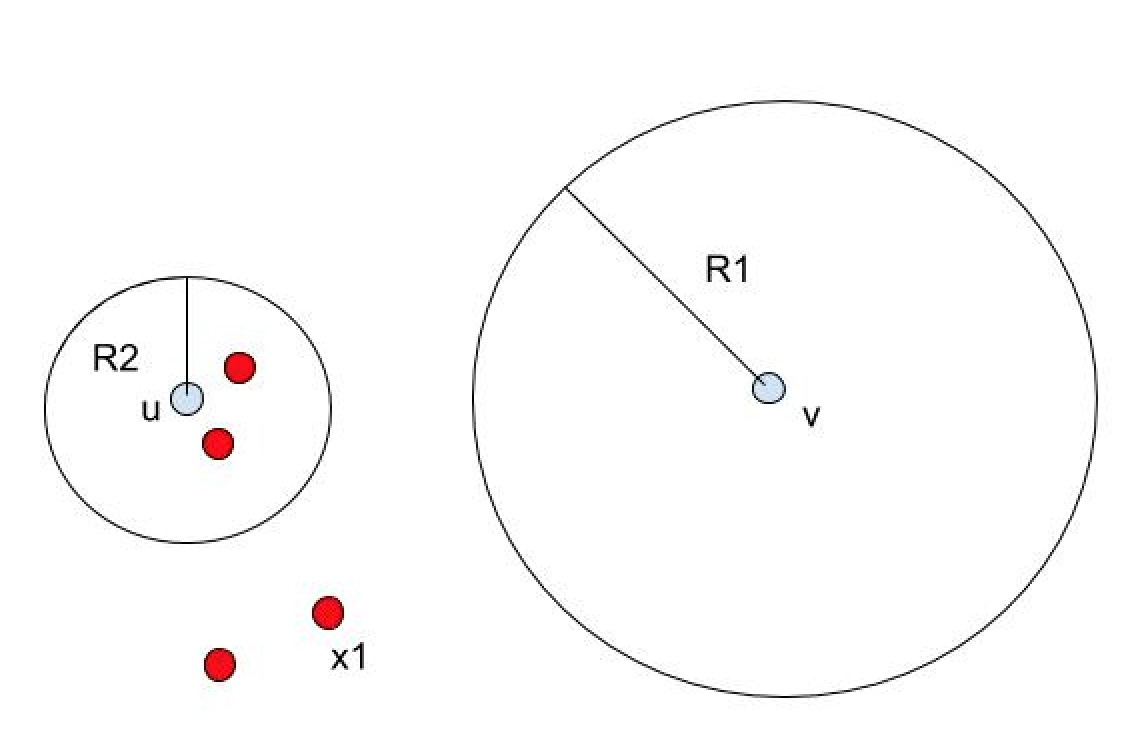
\includegraphics[width=0.5\textwidth]{chapter_5/files/construction.jpg}
\caption{An illustration of the construction in the proof}
\end{center}
\end{figure}

\textbf{Formal Proof}
\begin{proof}
  For $1 \leq i \leq \ceil{24 \sqrt{n} \ln n} = m$:
  \begin{enumerate}
  \item[1.] Pick $x \in \mathbf{X}$ with probability
    $\min (\frac{1}{2}, \frac{1}{\sqrt{n}})$  independently and thus
    constitute the set $A_i$.\\  
  \item[2.] Pick $x\in \mathbf{X}$ with probability $\min
    (\frac{1}{2}, \frac{1}{n})$ independently and thus constitute the
    set $\bar{A}_i$.
  \end{enumerate}

\[
\forall x \in \mathbf{X}, f(x)=
\begin{bmatrix}
    \rho (u,A_1)\\
    \rho (u,A_2)\\
    ...\\
    \rho (u,A_m)\\
    \rho (u,\bar{A}_1)\\
    \rho (u,\bar{A}_2)\\
    ...\\
    \rho (u,\bar{A}_m)\\
\end{bmatrix}
\]
\textbf{Claim}: Pick any $u,v \in \mathbf{X},u\neq v$ and pick $i$,
then either $|\rho (u,A)-\rho (v,A)| \geq \frac{1}{3} \rho (u,v)$ or
$|\rho (u,\bar{A})-\rho (v,\bar{A})|\geq \frac{1}{3} \rho (u,v)$ with
probability $\geq \frac{1}{12\sqrt{n}}$ (over the choices of $A$ and
$\bar{A}$). 

\begin{figure}[h!]
\begin{center}
\caption{An illustration of the three balls}
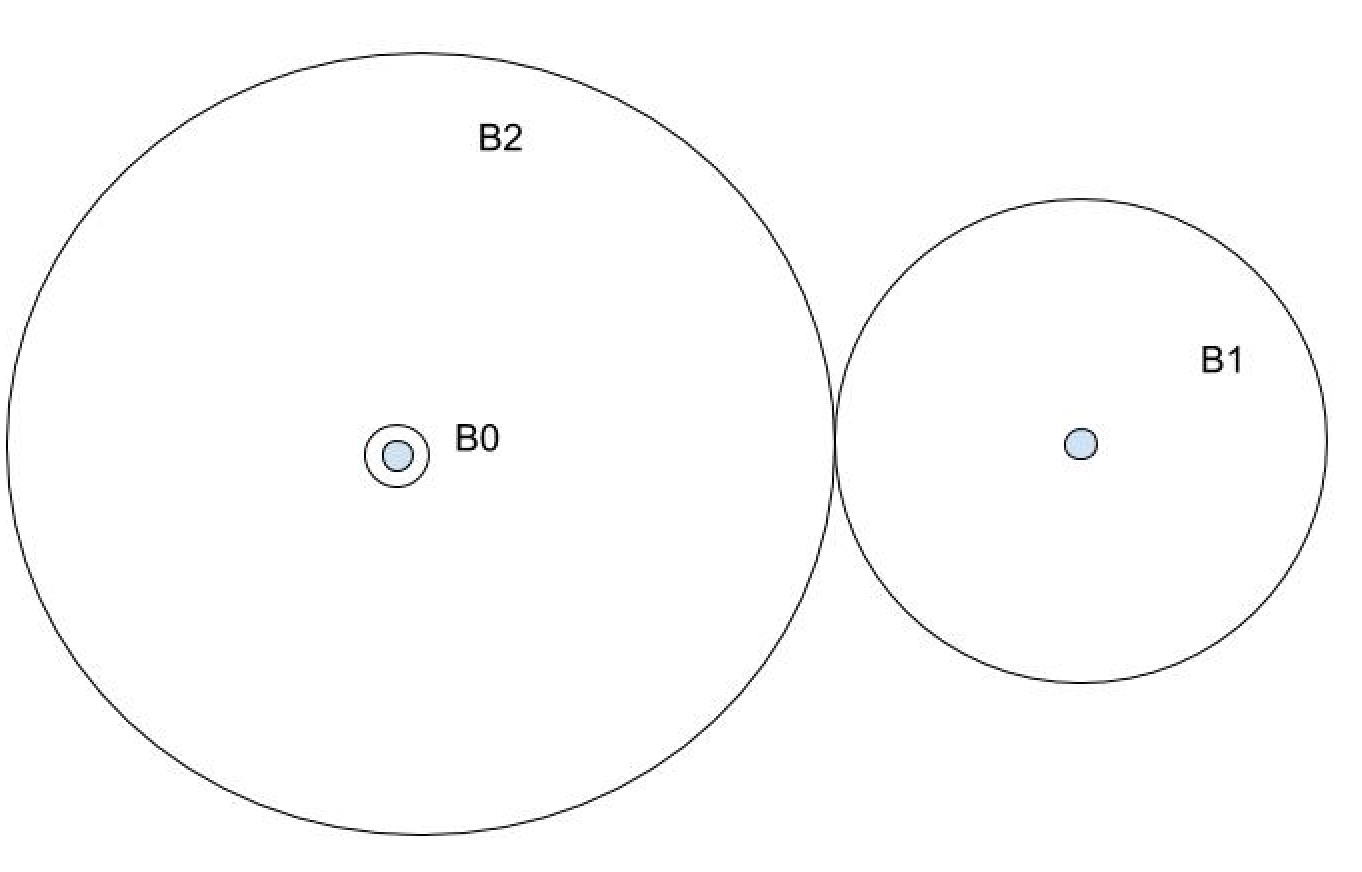
\includegraphics[width=0.5\textwidth]{chapter_5/files/three_balls.jpg}
\end{center}
\end{figure}
\begin{proof} (for the claim)
Assume we have three balls: $B_0(u,r=0)$, $B_1(v,r=\frac{1}{3}\rho
(u,v))$, $B_2(u,r=\frac{2}{3}\rho (u,v))$.\\ 
\textbf{Idea}: either $|B_1\cap \mathbf{X}|\leq \sqrt{n}$ (no points
from $B_1$ will be picked and at least one point from $B_0$ will be
picked with some probability) or $|B_1 \cap \mathbf{X}|>\sqrt{n}$ (no
points from $B_2$ will be picked and at least one point from $B_1$
will be picked with probability $\geq \frac{1}{12}\sqrt{n}$).\\ 
\textbf{Case1} ($|B_1\cap \mathbf{X}| \leq \sqrt{n}$):\\
Consider set $A$,\\
$Pr[E_1:=B_0 \cap A \neq \phi]=\min (\frac{1}{2}, \frac{1}{\sqrt{n}})$,\\
$Pr[E_2:=B_1\cap A=\phi]=(1-\min(\frac{1}{2},
\frac{1}{\sqrt{n}}))^{B_1\cap \mathbf{X}}\geq (1-\min(\frac{1}{2},
\frac{1}{\sqrt{n}}))^{\sqrt{n}} \geq \frac{1}{4}$,\\ 
Since $E_1$ and $E_2$ are disjoint,
\[
Pr[E_1 \cap E_2] \geq \min (\frac{1}{8},\frac{1}{4\sqrt{n}})\geq
\frac{1}{12\sqrt{n}}. 
\]
\textbf{Case2} ($|B_1\cap \mathbf{X}| > \sqrt{n}$):\\
Consider set $\bar{A}$,\\
$Pr[E_3:=B_1\cap \bar{A}\neq \phi] \geq ... \geq \frac{1}{3\sqrt{n}}$,\\
$Pr[E_4:=B_2\cap \bar{A}= \phi] \geq ... \geq \frac{1}{4}$,\\
$Pr[E_3\cap E_4]\geq \frac{1}{12\sqrt{n}}$.\\
Therefore, the claim is true.
\end{proof}
We have:
\begin{align*}
\Pr\bigg[\exists u,v \in \mathbf{X} \textrm{ s.t. } \forall
  A_i,\ \bar{A}_i,\\|\rho (u,A_i) &- \rho (v, A_i) | < \frac{1}{3}
  \rho (u,v) \textrm{ and } |\rho (u,\bar{A}_i) - \rho (v, \bar{A}_i)
  | < \frac{1}{3} \rho (u,v) \bigg]\\ 
&\leq \sum_{(u,v)\in \mathbf{X}\times \mathbf{X} \textrm{unordered
    pair}} (1-\frac{1}{12\sqrt{n}})^m \textrm{ because of the union
  bound}\\ 
&\leq \binom{n}{2} e^{-\frac{1}{12\sqrt{n}}m}\\
&\leq \binom{n}{2} e^{\ln \frac{1}{n^2}}\\
&\leq \binom{n}{2} \frac{1}{n^2}\\
&<1.
\end{align*}
The proof uses the fact that $m=\ceil{24 \sqrt{n}} \ln n$ and $(1-x)
\leq e^{x}$.\\ 
Therefore, the embedding $f$ exists.


\end{proof}
\textbf{Open question}: Is there a deterministic construction of
embedding into $l_\infty^d d = O(\sqrt{n}\ln n)$ with $D=3$? 

\begin{theorem}[\textbf{Generalization}]
Let $D=2q-1\geq 3$(be odd).Then any n-point metric space can be
$D$-embedded into $l_\infty^d$ where $d=O(q n^{1/q} \ln n)$. 
\end{theorem}

\subsubsection{Summary}
Frechet $l_\infty^d d=n d=\Omega (n),D<3$.\\
Bourgain $l_\infty^d,d=O(\sqrt{n}\ln n),D=3$.\\

\subsection{Embedding into $l_2^d$}
\textbf{Result1}: (follows from Bourgain generalization): Any
$n$-point metric space can be embedded into $l_\infty^d$ with
$D=O(\log^2 n)$ and $d=O(\log^2 n)$.\\  
\textbf{Refinement}(Bourgain's $l_2$ result): Any $n$-point metric can
embed in $l_2^d$ with $D=O(\log n)$.\\ 

\begin{theorem}[Johnson-Lidenstrauss "flatten" lemma(JL-lemma, 1984)]
Pick any $0<\epsilon<\frac{1}{2}$. Then for any integer $n$, let $d >
\ceil{\frac{4}{\epsilon^2} (2\ln n + \ln 3)} \rightarrow d > \Omega
(\frac{\ln n}{\epsilon^2})$. Then for any set $V \subset \mathbb{R}^D,
\ s.t. \ |V|=n$, there exists a map $f:\mathbb{R}^D \rightarrow
\mathbb{R}^d \ s.t. \ \forall u,v \in V, \ (1-\epsilon)||u-v||^2_2
\leq ||f(u)-f(v)||_2^2 \leq (1+\epsilon)||u-v||^2_2$.\\ 
\begin{itemize} 
\item Moreover, $f$ is simply a linear map.  
\item Pick a random $d$-dim subspace (in $D$-dim), then above holds 
  true with high probability(minor global scaling).  
\end{itemize} 
\end{theorem} 
For any $D$-dim $v$, define \[
f(v)=
\begin{bmatrix}
    x_{11}&...&x_{1D}\\
    ...\\
    x_{d1}&...&x_{dD}\\
\end{bmatrix}v
\]
where $x_{ij}\ \forall i,j$ is drawn from a Gaussian
independently. Then with high probability, $f$ satisfies the above
properties. 

$\exists \ n+1$ points in $\mathbb{R}^D (D\geq n)$ that cannot be
isometrically embeddable in $l_2^d$ with $d<n$.\\ 
\textbf{Application of JL}:
\begin{itemize}
\item Fast provable clusterings(1999)
\item Fast approximate nearest neighbor search
\item Approximate solutions to graph problems(e.g. multi-commodity
  flow) 
\item Fast approximate linear algebra(e.g. matrix
  multiplication)("sketching") 
\end{itemize}
\textbf{Proof Sketch}\\
Observation: Let $\phi$ be a random $d$-dim subspace (in $D$-dim).\\
\textbf{Claim}: We can show that $\mathbb{E}_\phi[||\phi
  (w)||^2]=\frac{d}{D}$. Pick any $0<\epsilon<\frac{1}{2}$ and fix a
unit vector $w\in \mathbb{R}^D$. Then,  
\[
\Pr\left[||\phi (w)||^2 < (1-\epsilon) \frac{d}{D} \textrm{ or }
  ||\phi (w)||^2 \geq (1+\epsilon) \frac{d}{D}\right] \leq
3e^{-d\epsilon^2/4}. 
\]
\emph{Note:} on average, a projection of $w$ onto the random subspace
$\phi$ has expected squared-norm: 
\[\E\left[||\phi(w)||^2\right] = \frac{d}{D}.\]
Then, apply a concentration/Chernoff-type bound.

\section{JL-Lemma}
\subsection{Recall}
\begin{theorem}[Johnson-Lidenstrauss ``flattening" lemma, 1984]
\noindent Pick any $0<\epsilon<\frac{1}{2}$. Then for any integer $n$,
let $d > \ceil{\frac{4}{\epsilon^2} (2\ln n + \ln 3)}$, that is, $d >
\Omega (\frac{\ln n}{\epsilon^2})$. Then for any set $V \subset
\mathbb{R}^D, \ s.t. \ |V|=n$, there exists a linear map
$f:\mathbb{R}^D \rightarrow \mathbb{R}^d \ s.t. \ \forall u,v \in V$,  

\begin{equation*}
(1-\epsilon)||u-v||^2_2 \leq ||f(u)-f(v)||_2^2 \leq
  (1+\epsilon)||u-v||^2_2 
\end{equation*}
\end{theorem}
\begin{remark} Since $\sqrt{1 - \epsilon} \leq 1 - \epsilon$ and $1 +
  \epsilon \leq \sqrt{1 + \epsilon}$, the embedding is thus a
  $D$-embedding where the distortion  $D=\frac{1+\epsilon}{1-\epsilon}
  \leq 1+5\epsilon$ because $\frac{1}{1-\epsilon} \leq 1+2\epsilon
  \ \forall 0 < \epsilon < \frac{1}{2}$. The above holds true for any
  random $d$-dim subspace (in $D$-dim) with high probability (minor
  global scaling). 
\end{remark}



\begin{lemma}[Concentration of Measure] \label{concentration}
Pick any $0<\epsilon<\frac{1}{2}$, fix any unit vector $w\in
\mathbb{R}^D (\mathrm{i.e.}~||w||=1)$, let
$\phi:\mathbb{R}^D\rightarrow \mathbb{R}^d$, $d<D$, be a random
subspace map. Then,  
\[\Pr_\phi \left[||\phi(w)||^2 < (1-\epsilon)\frac{d}{D} \textrm{ or }
  ||\phi (w)||^2 > (1+\epsilon)\frac{d}{D}\right]\leq 3 e^{-d
  \epsilon^2/4}.\] 
\end{lemma}

For JL, we'll want to project to a random subspace, then scale by $\sqrt{D/d}$.

\subsection{Proof of JL-Lemma}
\begin{proof}
Because $\phi$ is linear, there is a corresponding matrix $P\in
\mathbb{R}^{d\times D}$ s.t. $\phi(w)=Pw$. \\ 
$f:=\sqrt{\frac{D}{d}} \phi$, so $f(w) = \sqrt{\frac{D}{d}} Pw$. For
any distinct $u,v\in V$,\\ 
\begin{align*}
\Pr\bigg[\exists u,v \in V &\textrm{ s.t. } ||f(u)-f(v)||^2 <
  (1-\epsilon)||u-v||^2\textrm{ or } ||f(u)-f(v)||^2 >
  (1+\epsilon)||u-v||^2\bigg]\\ 
&\leq \sum_{\substack{(u,v)\in V\times V\\
    \mathrm{unordered~pairs}}} \Pr_\phi \Big[||f(u)-f(v)||^2 <
  (1-\epsilon)||u-v||^2\\  
&\hspace{4cm}\textrm{ or } \ \ ||f(u)-f(v)||^2 >
  (1+\epsilon)||u-v||^2\Big]\\ 
& = \sum_{\substack{(u,v)\in V\times V\\
                  \mathrm{unordered~pairs}}} \Pr_\phi
\bigg[\left|\left|\phi
  \left(\frac{u-v}{||u-v||}\right)\right|\right|^2 <
  (1-\epsilon)\frac{d}{D}\\ 
&\hspace{4cm}\textrm{ or }\ \ \left|\left|\phi
  \left(\frac{u-v}{||u-v||}\right)\right|\right|^2 >
  (1+\epsilon)\frac{d}{D}\bigg]\\ 
&\leq \binom{n}{2} 3 e^{-d\epsilon^2/4} < 1
\end{align*}
where the first inequality is a union bound, and the last inequality
holds if we choose $d$ such that: 
\[d > \left\lceil\frac{4}{\epsilon^2} (2\ln n + \ln 3)\right\rceil.\]
The inner inequality follows from the linearity of $f =
\sqrt{\frac{D}{d}} \phi$, followed by an application of
Lemma~\ref{concentration}: 
\begin{align*}
||f(u)-f(v)||^2 < (1-\epsilon)||u-v||^2
&\Leftrightarrow \norm{\sqrt{\frac{D}{d}}
  \phi\left(\frac{u-v}{||u-v||}\right)}^2 < (1-\epsilon)\\ 
&\Leftrightarrow \norm{\phi\left(\frac{u-v}{||u-v||}\right)}^2 <
(1-\epsilon)\frac{d}{D}. 
\end{align*}
\end{proof}

\noindent\textbf{Recap}: 

\begin{itemize}
\item JL is a linear dimensionality-reduction technique. The goal is
  to preserve $\ell_{2}$ distances up to distortions of $1\pm
  \epsilon$. 

\item This is also a concentration result, $\norm{\phi(w)}^{2} <
  (1-\epsilon)d/D$, where $||\phi(w)||^{2}$ is the actual length of a
  particular draw and $d/D$ is the expected length. The actual draw
  will be concentrated towards a specific value, typically the
  expected value.  

\end{itemize}


\subsection{Aside: A list of concentration inequalities}
\begin{centering}
Markov \\
Chebychev \\
Chernoff \\
Hoeffding \\
Bernstein \\
Effron-Stein \\
Azuma \\
Mcdiarmid \\
Talagrand \\
\end{centering}
